\chapter{\ifproject%
\ifenglish Project Structure and Methodology\else โครงสร้างและขั้นตอนการทำงาน\fi
\else%
\ifenglish Project Structure\else โครงสร้างของโครงงาน\fi
\fi
}

The two main components of this project: \RootOurs{} and \RootAI. The interaction flow and project structure are shown in Figure \ref{fig:project-structure}.

\begin{figure}[h!]
  \begin{center}
    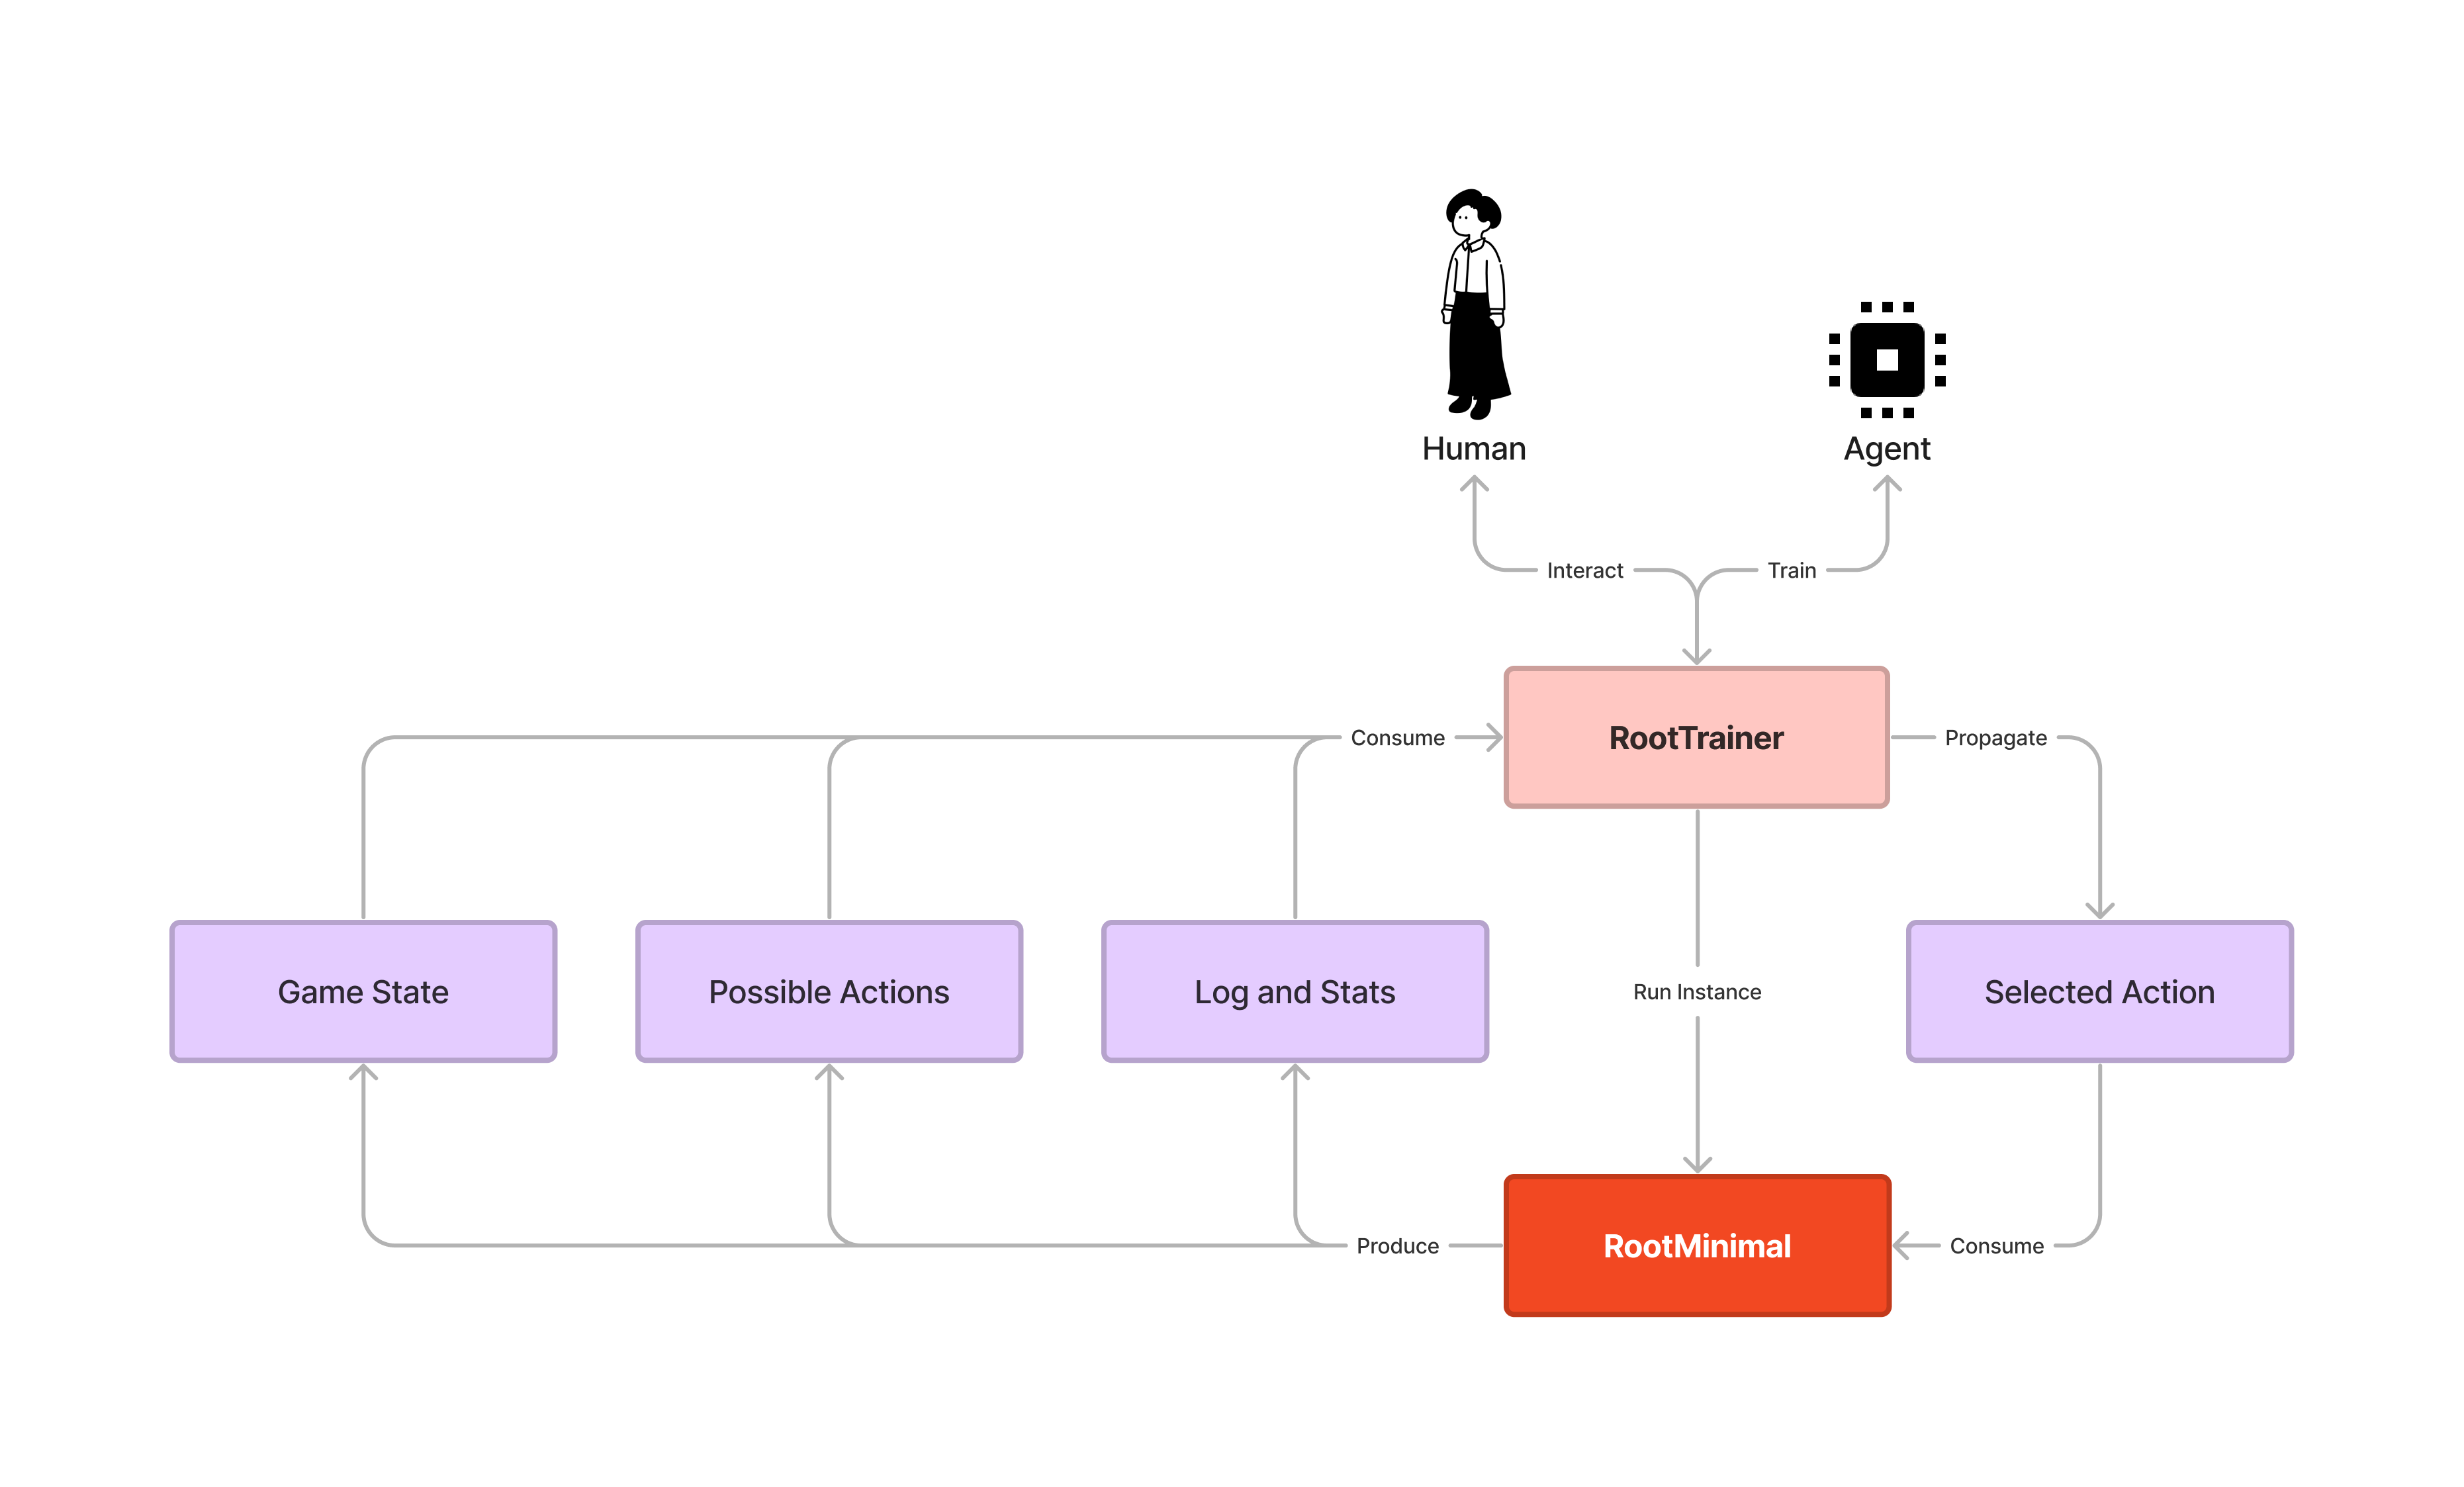
\includegraphics[width=\textwidth]{images/project-structure.png}
  \end{center}
  \caption{The project structure}
  \label{fig:project-structure}
\end{figure}

% ในบทนี้จะกล่าวถึงหลักการ และการออกแบบระบบ

\makeatletter

% \renewcommand\section{\@startsection {section}{1}{\z@}%
%                                    {13.5ex \@plus -1ex \@minus -.2ex}%
%                                    {2.3ex \@plus.2ex}%
%                                    {\normalfont\large\bfseries}}

\makeatother
%\vspace{2ex}
% \titleformat{\section}{\normalfont\bfseries}{\thesection}{1em}{}
% \titlespacing*{\section}{0pt}{10ex}{0pt}

\section{\RootOurs}
\RootOurs{} is the game environment that mimics \RootV{} in a game of \Marquise{} versus \Eyrie. It has the following features:
\begin{itemize}
  \item Simulate the current state of the game
  \item Generate all possible actions (``legal actions'') for the current player at the current state of the game
  \item Change state according to the selected action 
  % \begin{itemize}
  %   \item With option for whether the simulation will randomize the non-deterministic actions by itself or whether the player can input a specific outcome value for the non-deterministic actions.
  % \end{itemize}
\end{itemize}

% From P Khem's 
% This module enables other services to communicate with the dictionary. It performs querying
% words and adding new words on the request. There is only a single dictionary management
% system per back-end service. The system performs word querying and word modifying in
% the database, which the back-end service cannot do directly.
\section{\RootAI} \label{ch3-root-trainer}
\RootAI{} is the framework that allows humans and AI agents to interact with \RootOurs{} instance's environment.

There are 2 agent implementation methods: Random decision and Monte Carlo Tree Search (MCTS).

\subsection{Random decision}
The agent constructed using the random decision method will uniformly select an action from all legal actions at the current state. The list of legal actions has a \gls{discrete-uniform-distribution}, with each action having an equal likelihood of being chosen. % TODO: cite Wiki: discrete uniform distribution

% The agent built with random decision method will randomly select actions where all action has a uniform probability to be picked.

\subsection{Monte Carlo tree search (MCTS)} % TODO: add problem with current MCTS and Root
The agent will perform a tree search at the current state, determine which action has the highest probability of winning the game, and take that action. The winning probability of each action will be calculated using the MCTS approach.

% TODO: rework this sentence: "The winning probability of each action will be calculated using the MCTS approach."

\subsubsection{One-Depth MCTS}
``One-Depth MCTS'', similar to \textit{Flat Monte Carlo} \cite{mcts-survey}, is an MCTS agent that is implemented as a proof-of-concept for demonstrating that MCTS algorithm works with \RootB{}. It is called One-Depth because it only performs the legal action and then immediately rolls out from that state, not making any expansion down more than the first depth.

\subsubsection{General MCTS}
``General MCTS'' is the main MCTS algorithm in our project. The specific variant of MCTS called Open-Loop MCTS is used as the basis of implementation for this agent due to the nondeterministic mechanism in this board game and use the UCB policy as a tree policy.

General MCTS has multiple parameters which can be customized to create multiple variants of MCTS. There are 6 parameters that we implemented, including: \texttt{reward-function}, \texttt{expand-count}, \texttt{rollout-no}, \texttt{time-limit}, \texttt{action-count-limit}, and \texttt{best-action-policy}.

\begin{enumerate}
  \item \textbf{\texttt{reward-function}}: The MCTS must determine how ``good'' the state at the end of a rollout is. This is done using the reward-function. There are 4 options for this parameter:
  \begin{itemize}
    \item \texttt{win}: considers whether the player wins; 1 if win, 0 otherwise
    \item \texttt{vp-difference}: considers the VP differences of the current player and the enemy player; \texttt{vp\_player} - \texttt{vp\_enemy}
    \item \texttt{vp-difference-bin}: considers the VP differences is \texttt{d}; 1 if d > 0,  0 otherwise
    \item \texttt{vp-difference-relu}: considers the VP differences is \texttt{d}; \texttt{d} if \texttt{d} > 0, 0 otherwise  
  \end{itemize}
  \item \textbf{\texttt{expand-count}}: Whenever the MCTS expands the game tree, a node is added to the tree. This parameter limits the number of expansions. The expansion could go on indefinitely until the entire tree is searched, which should result in a better outcome, but that would take too much computation time. That is the reason that this parameter exists.
  \item \textbf{\texttt{rollout-no}}: Whenever the MCTS expands, it must perform a number rollouts to determine the reward of that node. This parameter controls the amount of rollouts per node. A rollout is bound to come across some nondeterministic actions which could result in varying outcome of that rollout. Multiple rollouts per node can be used to help mitigate the varying outcomes.
  \item \textbf{\texttt{time-limit}}: A rollout may encounter an infinite loop or may take a very long time. This parameter controls the time limit for each rollout. A rollout will immediately stop at its current state if a time limit is exceeded. % Note that from our experience, a rollout is pretty fast.
  \item \textbf{\texttt{action-count-limit}}: A rollout does not necessarily need to reach a game-ending state to stop. This parameter controls how many actions will be executed before stopping a rollout, i.e., how deep into the future will a rollout look.
  \item \textbf{\texttt{best-action-policy}}: As described in Section \ref{winning-action}, when the MCTS algorithm finishes, it must choose which legal action is the best. This parameter controls how the ``best'' legal action is picked. There are 4 options for this parameter:
  \begin{itemize}
    \item \texttt{max}: picks the legal action with the highest reward
    \item \texttt{robust}: picks the most visited legal action
    \item \texttt{UCB}: picks the legal action that maximises the upper confidence bound
    \item \texttt{secure}: picks the legal action that maximises the lower confidence bound
  \end{itemize}
\end{enumerate}

% TODO: add citations to UCB, secure

% \subsection{Reinforcement learning neural network (RLNN)}
% The agent constructed using RLNN will use RNN type model, taking the current state, past states, and past actions as input and outputing the probability of choosing each action from all legal actions in the current state. Then calculate the reward of that action using the reward function, which is yet to be defined. Adjust the neural network according to the reward, and adjust the agent’s current state to the new state in the feedback. % unconfirmed


% \begin{enumerate}
%   \item Agent: the player that's playing as \Marquise{} faction or \Eyrie{} faction
%   \item Environment: the map, opponent's state and action, draw pile, etc. in \RootOurs % not sure
%   \item State: all game components that belonged to the player
%   \item Reward: victory points earned, getting a win, or taking hold of clearing with matching suit to the played dominance card, all combined together through the reward function 
%   \item Policy: the neural network
% \end{enumerate}

% TODO: add evaluation method